% !TEX root = Master.tex

The same strategy as in the previous subsection (\ref{sssec:kcc_26}) shall be followed. In \autoref{fig:scatter_res_kcc_28}, a lower tail dependence can be suspected. Whether both positive and negative dependencies are hiding in the the data is being tested beforehand, so that we can narrow down the number of plausible copula families.
\\

\begin{figure}[H]
\centering
  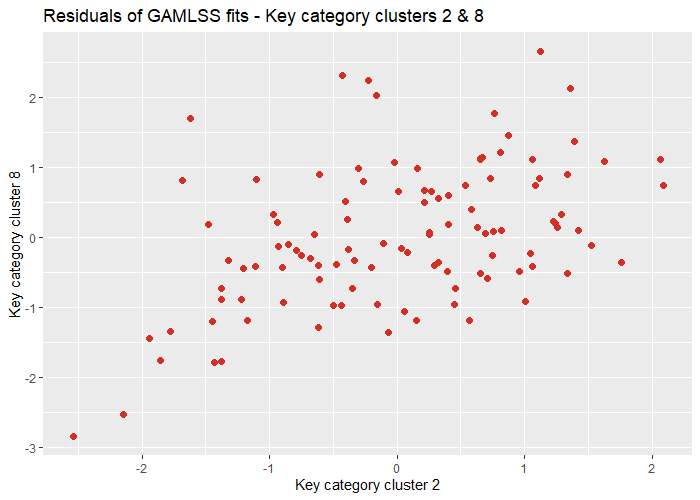
\includegraphics[width=0.45\linewidth]{figures/scatter_res_kcc_28.png}
  \caption{Scatterplot of estimated residuals of GAMLSS fits for key category clusters 2 \& 8}
  \label{fig:scatter_res_kcc_28}
\end{figure}


A \ac{GJRM} approach equivalent to Model \ref{eq:gjrm_formula_26} is applied here, with the only difference that we leave out the promo type (see Model \ref{eq:gjrm_formula_28}) since it not only has a non-significant effect, but unlike for the previous pair it also heavily distorts the outcome for this pair. 
\begin{equation}
\begin{array}{c}
\mu_{KCC 2}=\beta_{\mu,KCC2} \qquad \mu_{KCC 6}=\beta_{\mu,KCC6}  \\  \noalign{\vskip5pt}

log(\sigma_{KCC 2})=\beta_{\sigma,KCC2} \qquad log(\sigma_{KCC 6})=\beta_{\sigma,KCC6} \\  \noalign{\vskip5pt}

log(\nu) = \beta_{\nu} \\  \noalign{\vskip5pt}

tanh^{-1}(\theta)=\beta_{\theta}  +f(\textit{time})
\end{array}
\label{eq:gjrm_formula_28}
\end{equation} 
All model parameters but the copula parameter are set as constants. Since a t-copula is again applied, the copula parameter obtains an inverse hyperbolic tangent function as link. Also, time is the only covariate in Model \ref{eq:gjrm_formula_28}. \\
A summary about the coefficients of the estimated copula parameter $\hat{\theta}$ is printed in \autoref{tab:theta_coeff_kcc_28}.  We first examine copulas which account for positive as well as negative dependencies.\footnote{With the help of the \textit{BiCopSelect()} function of the \textit{VineCopula} package \citep{nagler2019vinecopula}.} The t-copula is again the most appropriate within a set of copula families including the independence copula, the Gaussian copula, the Student's t-copula and the Frank copula. Looking at \autoref{tab:theta_coeff_kcc_28}, we can see that time has a significant non-linear effect on $\hat{\theta}$ (18.50 edf) and its partial smooth effect can be checked visually in \autoref{fig:time_effect_on_theta_28}.
\\



\begin{table}[H]
\centering
\begin{tabular}{l|c|c|c|c}
\hline
                               \textbf{$\hat{\theta}$ Coefficients}       & \textbf{Estimate} & \textbf{Std. Error} & \textbf{z value} & \textbf{p-value}  \\ \hline\hline
$\beta_{\theta}$ \textit{(Intercept)}                  & 0.64     & 0.11       & 5.82    & 0.00 ***   \\ \hline
& & & & \\ \hline
\textbf{Smooth components}            & \textbf{edf}      & \textbf{Ref.df}     & \textbf{Chi.sq}  & \textbf{p-value}  \\ \hline\hline
\textit{$f$(time)}                 & 18.50    & 21.75      & 41.44   & 0.01 ** \\ \hline
\end{tabular}
\caption{Estimated $\hat{\theta}$ coefficients of \ac{GJRM} fit on key category clusters 2 \& 8}
\label{tab:theta_coeff_kcc_28}
\end{table}











\begin{figure}[H]
\centering
  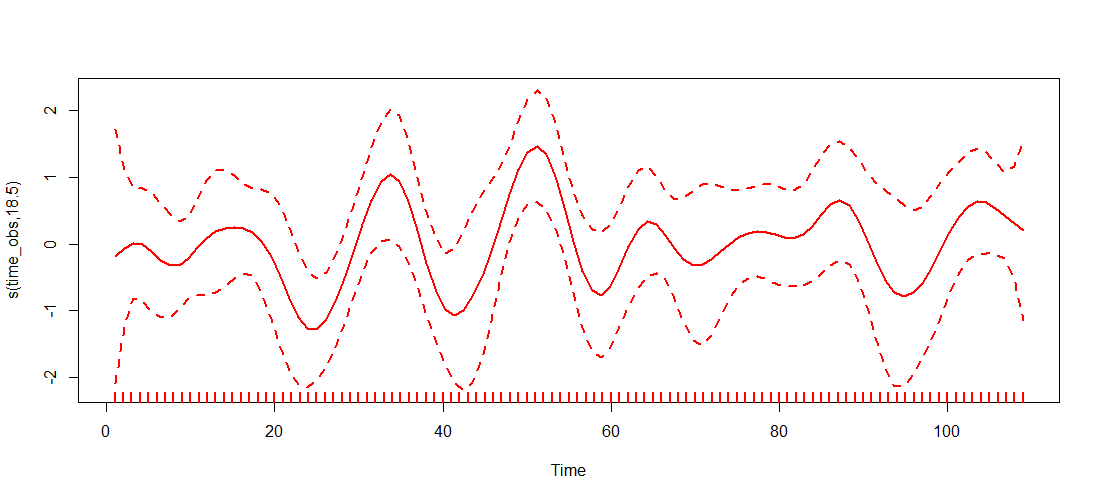
\includegraphics[width=0.95\linewidth]{figures/time_effect_on_theta_28.png}
  \caption{Estimated Smooth effect of time on the copula parameter $\theta$ with 95\% confidence bands for key category clusters 2 \& 8}
  \label{fig:time_effect_on_theta_28}
\end{figure}





\begin{figure}[H]
\centering
  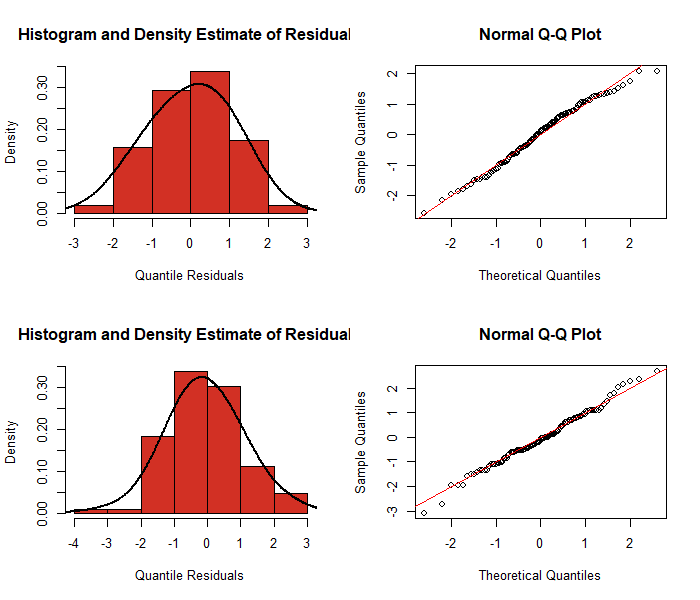
\includegraphics[width=0.80\linewidth]{figures/res_hist_qqplot_28.png}
  \caption{Diagnostic plots of quantile residuals based on \ac{GJRM} models for key category clusters 2 \& 8}
  \label{fig:res_hist_qqplot_28}
\end{figure}

The parsimonious model setup produces a nice fit. The quantile residuals are remarkably close to a standard normal distribution, which is reflected in the histograms and QQ-plots of both margins in \autoref{fig:res_hist_qqplot_28}.\\
Consequently, we proceed to analyzing the correlation parameter. Once again, $\hat{\theta}$ takes on positive as well as negative values interchangeably over time periods. Therefore, considering further copula families like the Clayton copula would be arguably inappropriate.
\\


Looking at the correlation structure in \autoref{fig:estimated_theta_kcc_28}, we can see that during both mid-seasons of Fall-Winter 2017 and 2018 there is some negative dependence between the two clusters. End of Spring-Summer 2017 and beginning of Spring-Summer 2018 also show some negative correlation.
\\

\begin{figure}[H]
\centering
  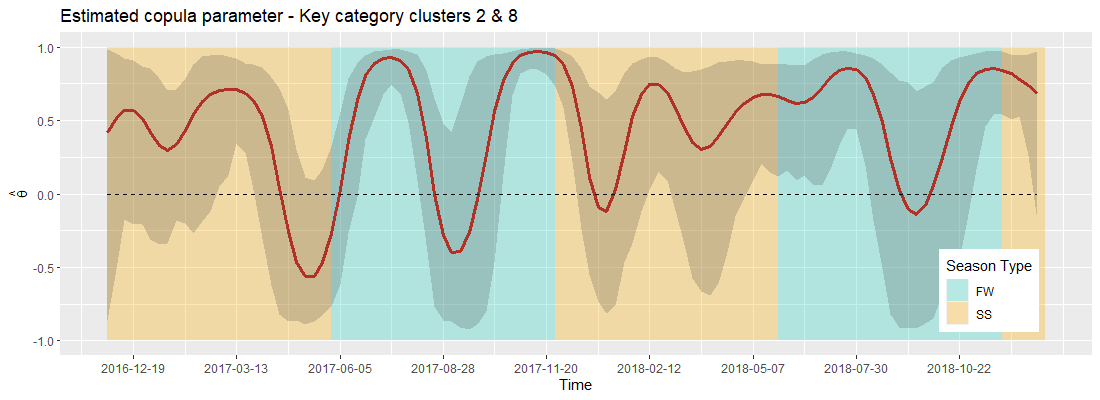
\includegraphics[width=0.95\linewidth]{figures/estimated_theta_kcc_28.png}
  \caption{Estimated copula parameter over time and 95\% confidence bands from a \ac{GJRM} t-copula model with normal margins for key category clusters 2 \& 8 - Season type in the background - Dashed horizontal line at $\hat{\theta} = 0$}
  \label{fig:estimated_theta_kcc_28}
\end{figure}
%  - Confidence bands are neglected for clarity of the graph














%On this \ac{KCC} pair, the \ac{GJRM} approach is not as favorable as in the pair KCC 2 \& KCC 6, though it might be considered acceptable (\autoref{fig:margin_estimates_kcc_28}).  \\
%
%\begin{figure}[H]
%\centering
%  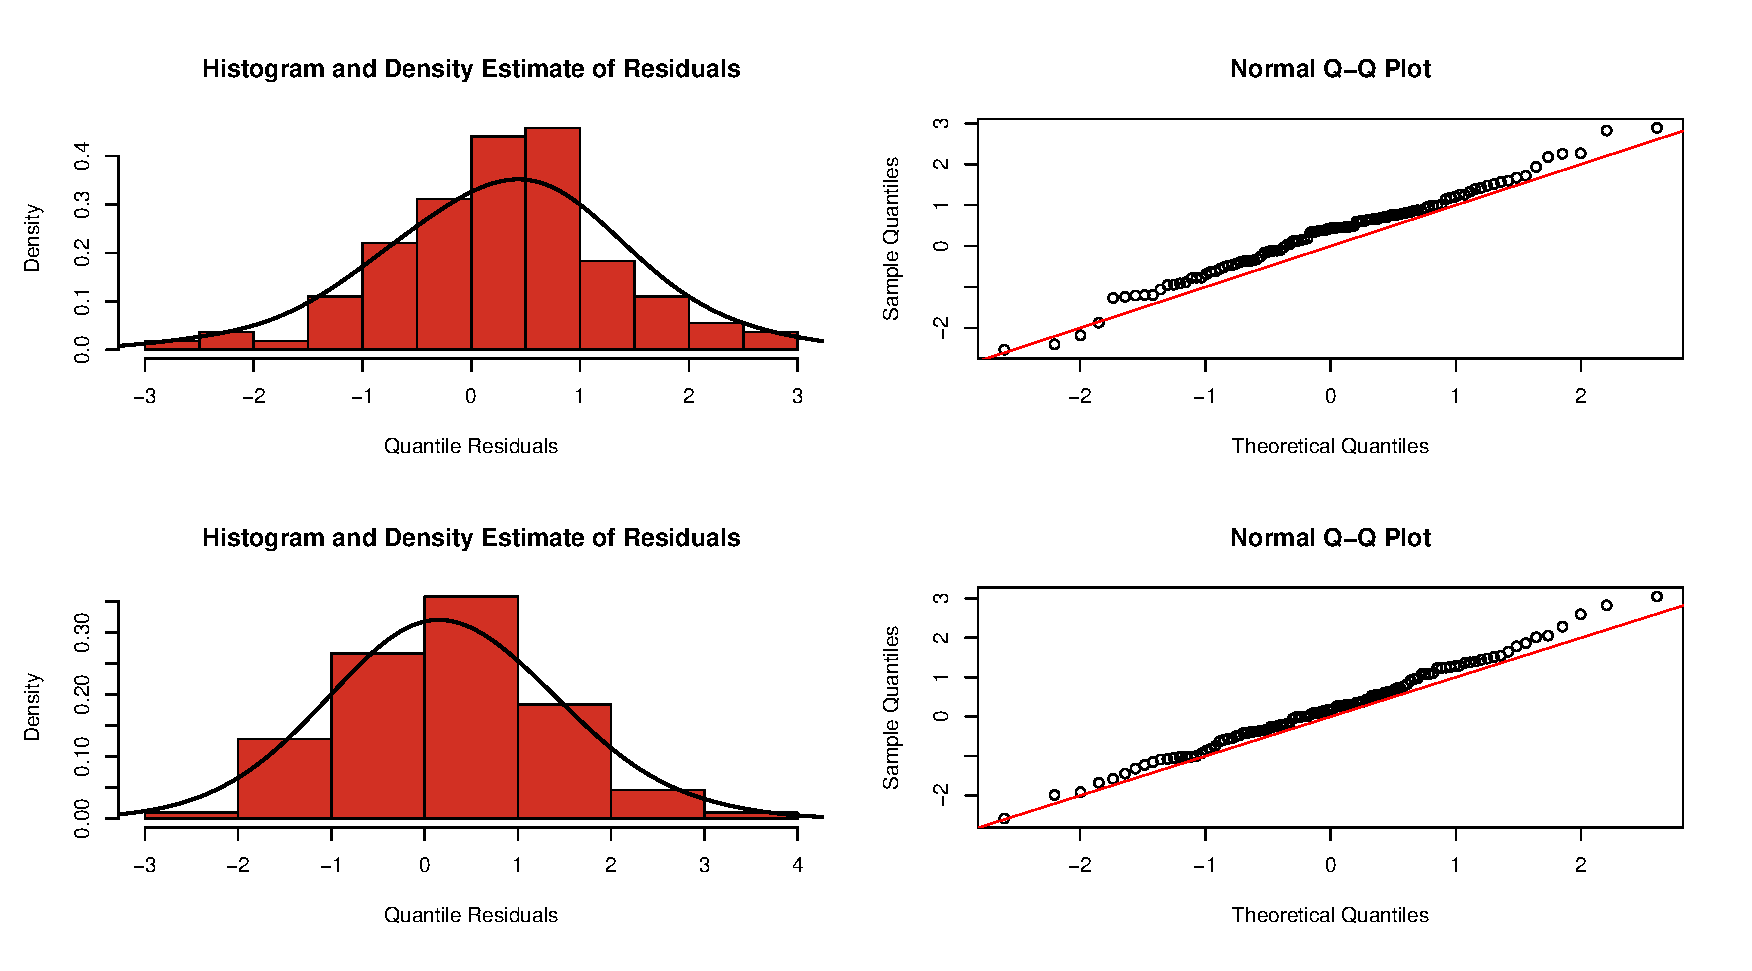
\includegraphics[width=0.9\linewidth]{figures/margin_estimates_kcc_28.eps}
%  \caption{Estimation diagnostics for the response margins KCC 2 \& KCC 8; \ac{GJRM} approach}
%  \label{fig:margin_estimates_kcc_28}
%\end{figure}
%
%This circumstance is reflected within the comparison of the "gamCopula" estimated dependence measures. The overall similarity between the two lines in \autoref{fig:copula_parameters_28}, which depict the time-dependent correlation parameters of this pair, is given. However, the details reveal that there are severe differences between the estimation methods. As the gamCopula approach yields converge in contrast to the \ac{GJRM} method, it might be preferential. Nevertheless, the results should be treated with adequate caution.
%
%\begin{figure}[H]
%\centering
%  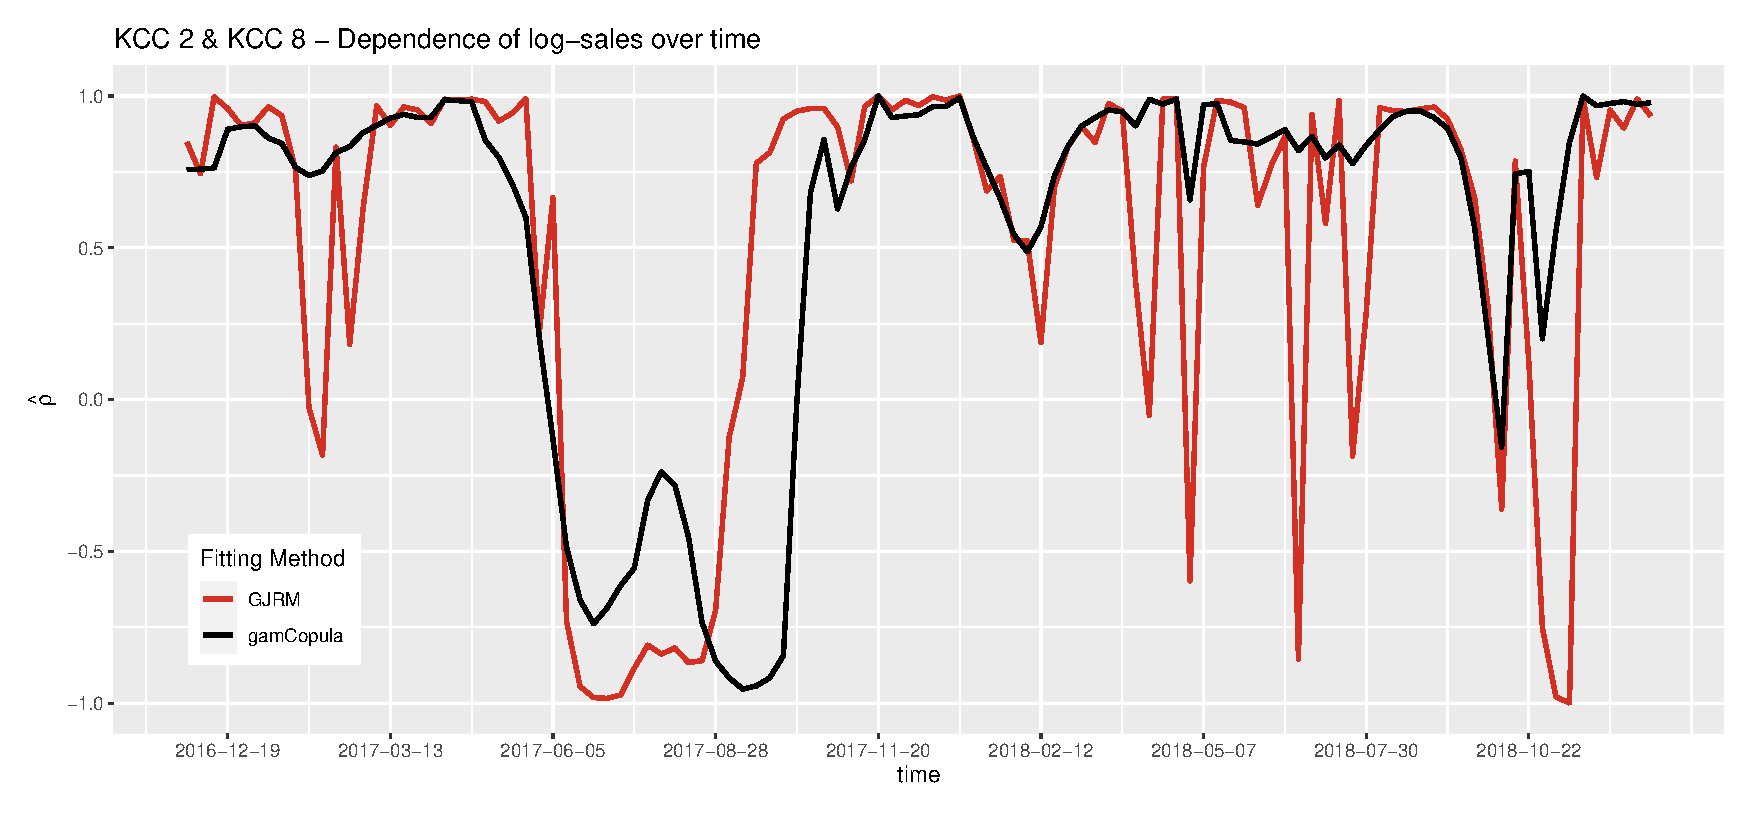
\includegraphics[width=0.9\linewidth]{figures/copula_parameters_28.eps}
%  \caption{Estimated time-varying Pearson's correlation coefficients for the pair KCC 2 \& KCC 8}
%  \label{fig:copula_parameters_28}
%\end{figure}
%
%
%The stretched sign change of the correlation over time happens, just like in the previous pair, from June to August 2017. The curves here are surprisingly different in terms of their stability. The gamCopula method seems to have a more stable course compared to the \ac{GJRM} approach. The red line in \autoref{fig:copula_parameters_28} appears very sensitive in very short time intervals.



